% Hlavicka pro protokoly z fyzikalniho praktika.
% Verze pro: LaTeX
% Verze hlavicky: 22. 2. 2007
% Autor: Ustav fyziky kondenzovanych latek
% Ke stazeni: www.physics.muni.cz/ufkl/Vyuka/
% Licence: volne k pouziti, nejlepe k vcasnemu odevzdani protokolu z Vaseho mereni.

\documentclass[a4paper,11pt]{article}

% Kodovani (cestiny) v dokumentu: utf-8
%\usepackage[cp1250]{inputenc}	% Omezena stredoevropska kodova stranka, pouze MSW.
\usepackage[utf8]{inputenc}	% Doporucujeme pouzivat UTF-8 (unicode).
\usepackage[T1]{fontenc}
\usepackage{lmodern}

%%% Nemente:
\usepackage[margin=2cm]{geometry}
\newtoks\jmenopraktika \newtoks\jmeno \newtoks\datum
\newtoks\obor \newtoks\skupina \newtoks\rocnik \newtoks\semestr
\newtoks\cisloulohy \newtoks\jmenoulohy
\newtoks\tlak \newtoks\teplota \newtoks\vlhkost
\usepackage{amsmath}
\usepackage{mathtools}
\usepackage{graphicx}
\usepackage{multirow}

\usepackage{pgfplotstable} 
\usepackage{booktabs}

\graphicspath{ {./images/} }
%%% Nemente - konec.


%%%%%%%%%%% Doplnte pozadovane polozky:

\jmenopraktika={Fyzikální praktikum 3}  % nahradte jmenem vaseho predmetu
\jmeno={Artem Gorodilov}            % nahradte jmenem mericiho
\datum={5. ~června  2024}        % nahradte datem mereni ulohy
\obor={Astrofyzika}                     % nahradte zkratkou vami studovaneho oboru
\skupina={Po 14:00}            % nahradte dobou vyuky vasi seminarni skupiny
\rocnik={II}                  % nahradte rocnikem, ve kterem studujete
\semestr={II}                 % nahradte semestrem, ve kterem studujete

\cisloulohy={E}               % nahradte cislem merene ulohy
\jmenoulohy={Zeemanův jev} % nahradte jmenem merene ulohy

\tlak={979}                   % nahradte tlakem pri mereni (v hPa)
\teplota={21.4}               % nahradte teplotou pri mereni (ve stupnich Celsia)
\vlhkost={46}               % nahradte vlhkosti vzduchu pri mereni (v %)

%%%%%%%%%%% Konec pozadovanych polozek.


%%%%%%%%%%% Uzitecne balicky:
\usepackage[czech]{babel}
\usepackage{graphicx}
\usepackage{amsmath}
\usepackage{xspace}
\usepackage{url}
\usepackage{indentfirst}
\usepackage{listings}
\usepackage{subcaption}
\usepackage{caption}
\usepackage{tabularx}
\usepackage[labelformat=parens,labelsep=quad,skip=3pt]{caption}

%%%%%% Zamezeni parchantu:
\widowpenalty 10000 \clubpenalty 10000 \displaywidowpenalty 10000
%%%%%% Parametry pro moznost vsazeni vetsiho poctu obrazku na stranku
\setcounter{topnumber}{3}	  % max. pocet floatu nahore (specifikace t)
\setcounter{bottomnumber}{3}	  % max. pocet floatu dole (specifikace b)
\setcounter{totalnumber}{6}	  % max. pocet floatu na strance celkem
\renewcommand\topfraction{0.9}	  % max podil stranky pro floaty nahore
\renewcommand\bottomfraction{0.9} % max podil stranky pro floaty dole
\renewcommand\textfraction{0.1}	  % min podil stranky, ktery musi obsahovat text
\intextsep=8mm \textfloatsep=8mm  %\intextsep pro ulozeni [h] floatu a \textfloatsep pro [b] or [t]

% Tecky za cisly sekci:
\renewcommand{\thesection}{\arabic{section}.}
\renewcommand{\thesubsection}{\thesection\arabic{subsection}.}
% Jednopismenna mezera mezi cislem a nazvem kapitoly:
\makeatletter \def\@seccntformat#1{\csname the#1\endcsname\hspace{1ex}} \makeatother

\begin{document}

\thispagestyle{empty}

{
\begin{center}
\sf 
{\Large Ústav fyzikální elektroniky PřF MU} \\
\bigskip
{\huge \bfseries FYZIKÁLNÍ PRAKTIKUM} \\
\bigskip
{\Large \the\jmenopraktika}
\end{center}

\bigskip

\sf
\noindent
\setlength{\arrayrulewidth}{1pt}
\begin{tabular*}{\textwidth}{@{\extracolsep{\fill}} l l}
\large {\bfseries Zpracoval:}  \the\jmeno & \large  {\bfseries Naměřeno:} \the\datum\\[2mm]
\large  {\bfseries Obor:} \the\obor  \hspace{40mm}  {\bfseries Skupina:} \the\skupina %
%{\bfseries Ročník:} \the\rocnik \hspace{5mm} {\bfseries Semestr:} \the\semestr  
&\large {\bfseries Testováno:}\\
\\
\hline
\end{tabular*}
}

\bigskip

{
\sf
\noindent \begin{tabular}{p{3cm} p{0.6\textwidth}}
\Large  Úloha č. {\bfseries \the\cisloulohy:} \par
\smallskip
% $T=\the\teplota$~$^\circ$C \par
% $p=\the\tlak$~hPa \par
% $\varphi=\the\vlhkost$~\%
&\Large \bfseries \the\jmenoulohy  \\[2mm]
\end{tabular}
}

\vskip0pt
    \begin{minipage}[t]{0.5\textwidth} 
        \section{Zadání}    
            \begin{enumerate}
                \item Ověřit funkci Fabry-Perotova interferometru. Ukazát, že naměřené poloměry různých interferenčních kroužků jedné vlnové délky souhlasí s vhodným vztahem uvedeným v návodu.
                \item Pomocí posunu vlnočtů při normálním Zeemanově jevu zjistit velikost Bohrova magnetonu.
                \item Zjistit, které složky rozštěpených spektrálních čar jsou vyzařovány ve směru kolmém na indukci magnetického pole, a které ve směru rovnoběžném. Změřit, jak jsou jednotlivé složky rozštěpených spektrálních čar polarizovány. Polarizaci stanovit pro oba směry záření (kolmý i rovnoběžný k magnetické indukci) a pro normální i anomální Zeemanův jev.
            \end{enumerate}
        \section{Teorie}
            \subsection{Zeemanův jev}
                Zeemanův jev je rozštěpení spektrálních čar v magnetickém poli. Rozštěpení je způsobeno interakcí mezi magnetickým dipólovým momentem atomu a magnetickým polem. Rozštěpení spektrálních čar je dáno vztahem:
                \begin{equation}
                    E_{mJ1} - E_{mJ2} = (m_{J2} g_{J2} - m_{J1} g_{J1}) \mu_B B
                \end{equation}
                kde $E_{mJ1}$ a $E_{mJ2}$ jsou energie stavů s magnetickými kvantovými čísly $m_{J1}$ a $m_{J2}$, $g_{J1}$ a $g_{J2}$ jsou Landého faktory, $\mu_B$ je Bohrův magneton a $B$ je magnetická indukce.
    \end{minipage}
    \hspace{10pt}
    \begin{minipage}[t]{0.5\textwidth} 
            \subsection{Fabry-Perotův interferometr}
                Pro analýzu spektrálních čar v magnetickém poli se používá Fabry-Perotův interferometr. Fabry-Perotův interferometr je optický přístroj, který využívá interference světla k měření vlnových délek. 
                \par Rozdíl druhých mocnin poloměrů interferenčních kroužků ($r_a$ a $r_b$) pro dvě vlnové délky s blízkými hodnotami vlnočtu ($\tilde{\lambda_a}$ a $\tilde{\lambda_b}$) je dán vztahem:
                \begin{equation}
                    r_{a,p+1}^2 - r_{a,p}^2 = 2(fZn)^2 \frac{1}{2nd\tilde{\lambda_a}}
                \end{equation} 
                kde $f$ je ohnisková vzdálenost čočky, $Z$ je zvětšení, $n$ je index lomu pro $\lambda_a$ a $d$ je tloušťka interferometru.
                \par Pro určení Bohrova magnetonu se využívá vztah:
                \begin{equation}
                    \mu_B = \frac{r_{a,p+1}^2 - r_{a,p}^2}{r_{b,p}^2 - r_{a,p}^2} \frac{hc}{2ndB}
                \end{equation}
                kde první index $i$ v $r_{i,p}$ označuje hlavní spektrální čáru (může nabývat hodnot $a$, $b$ a $c$) a druhý index $p$ označuje rozložené spektrální čáry (může nabývat hodnot $1$, $2$ a $3$). Podrobnosti jsou uvedeny na obrázku (\ref{fig:scheme}).

                \vspace{10pt}   
                \par \centering
                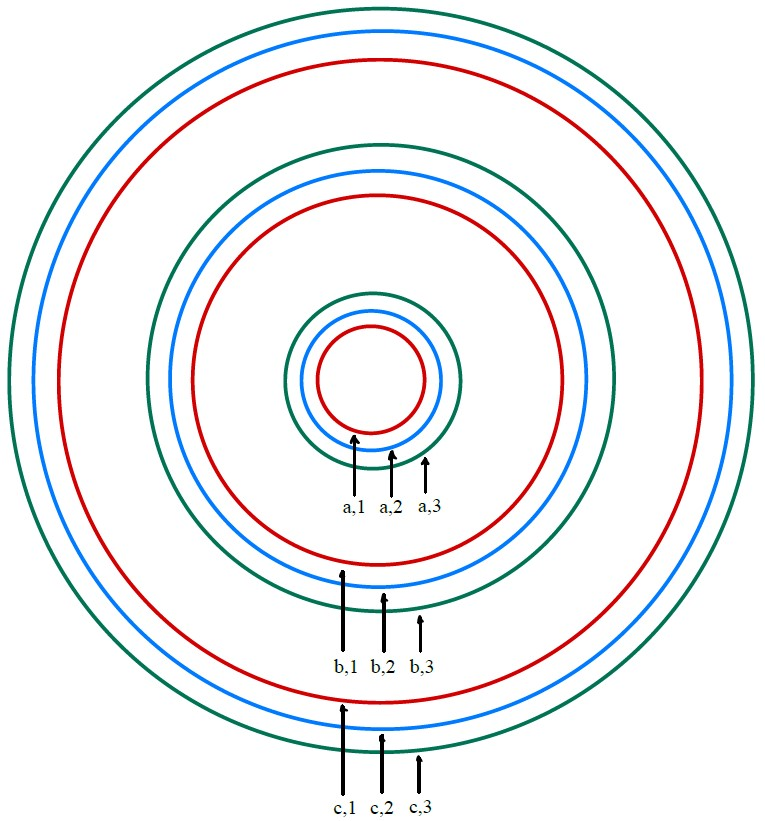
\includegraphics[scale=0.3]{scheme}
                \captionsetup{justification=centering, font=footnotesize}
                \captionof{figure}{Schéma rozložení spektrálních čar.}
                \label{fig:scheme}
                \vspace{10pt}
                \raggedright 
    \end{minipage}
\newpage
    \begin{minipage}[t]{0.5\textwidth} 
        \section{Měření}   
            \subsection{Ověření funkce Fabry-Perotůva interferometru}
                \par Pro ověření funkce Fabry-Perotova interferometru jsme změřili poloměry interferenčních kroužků pro spektrální čáry. Dále jsme vykreslili závislost druhé mocniny poloměru kružnic na jejich pořadí $f$ = $r^2(p)$. Poté jsme provedli lineární fitování dat, čímž jsme potvrdili lineární charakter této závislosti. Údaje jsou uvedeny v tabulce (1) a na grafu (\ref{fig:B_1}). Koeficient úměrnosti $\alpha$: 

                \begin{center}
                    $\alpha$ = 0.081(1) $\left[\frac{1}{mm^2}\right]$
                \end{center}

                \vspace{10pt}   
                \par \centering
                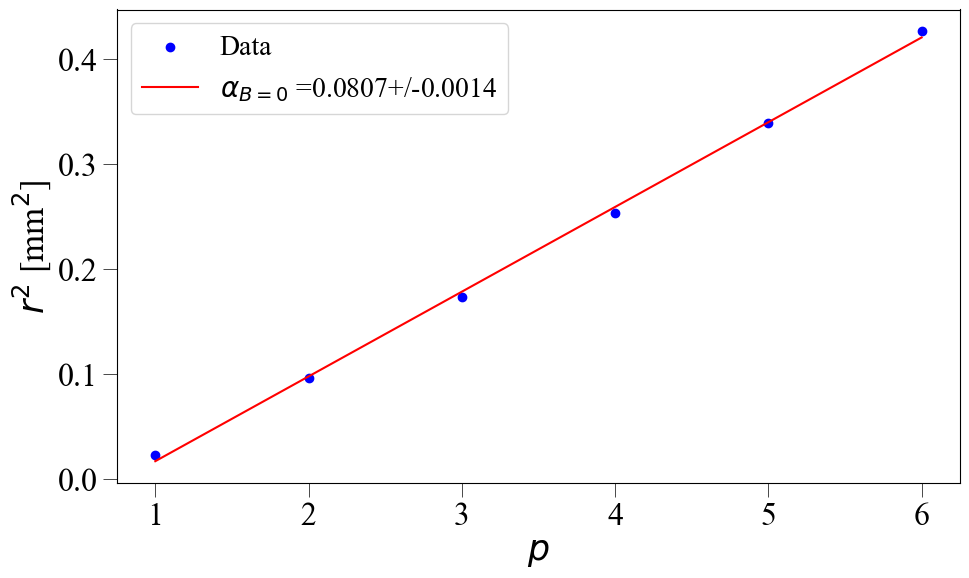
\includegraphics[scale=0.33]{B_1}
                \captionsetup{justification=centering, font=footnotesize}
                \captionof{figure}{Závislost druhé mocniny poloměru interferenčních kroužků $r^2$ na pořadí $p$.}
                \label{fig:B_1}
                \vspace{10pt}
                \raggedright

            \subsection{Bohrův magneton}
                \par Poté jsme použili údaje o závislosti $f$=$B(I)$, které nám byly poskytnuty. Provedli jsme fitování polynomem třetího stupně, čímž jsme interpolovali data na hodnoty $I$ od 0 A do 10 A. Údaje jsou uvedeny v tabulce (2) a na grafu (\ref{fig:I_B}).
            
                \vspace{10pt}   
                \par \centering
                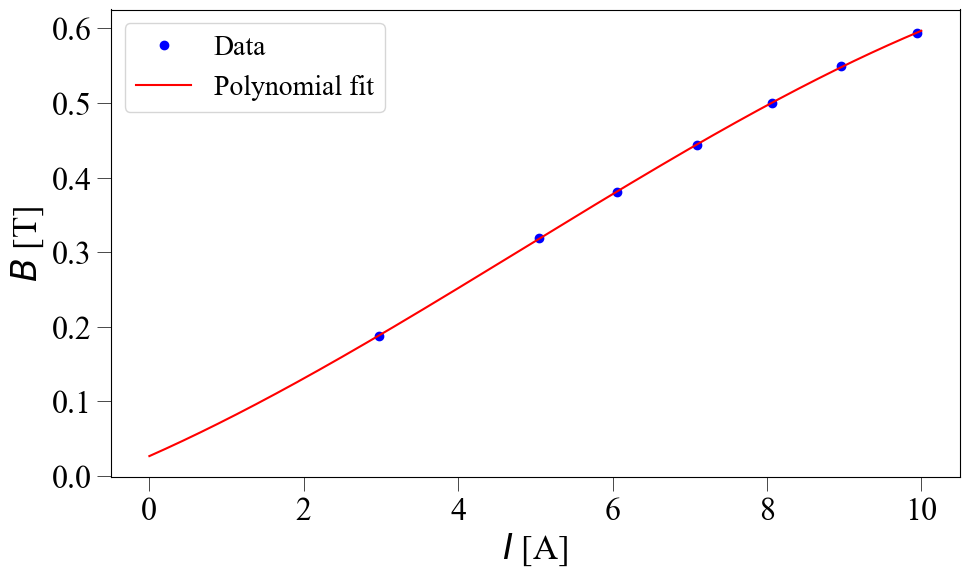
\includegraphics[scale=0.33]{I_B}
                \captionsetup{justification=centering, font=footnotesize}
                \captionof{figure}{Závislost magnetické indukce $B$ na proudu $I$.}
                \label{fig:I_B}
                \vspace{10pt}
                \raggedright 

                \par Dále zvýšením hodnoty proudu $I$ na cívce a následně zvýšením hodnoty magnetické indukce $B$ bylo zjištěno, že rozdělení spektrálních čar se projeví při hodnotách $I$ > 3.15 A, tj. $B$ > 199 mT. 
                
    \end{minipage}
    \hspace{10pt}
    \begin{minipage}[t]{0.5\textwidth} 
                Pomocí vzorce (3) jsme vypočítali hodnoty Bohrova magnetonu pro dvojice spektrálních čar $ab$ a $bc$ (viz obr. (1)). Tabulkové údaje pro výpočty:
                \begin{center}
                    $d$ = 3 [mm] ,~ $n$ = 1.456 \\
                \end{center}
                
                Pro každou dvojici spektrálních čar jsme získali dvě hodnoty $\mu_{B,ab}$ a $\mu_{B,bc}$. Údaje jsou uvedeny v tabulkách (3)-(10) a na grafu (\ref{fig:mu}).
                \par Po výpočtech jsme zjistili hodnotu $\mu_B$:
                \begin{center}
                    $\mu_B$ = 9.8(5) $\times 10^{-24}$ [J/T]
                \end{center}

                \vspace{10pt}   
                \par \centering
                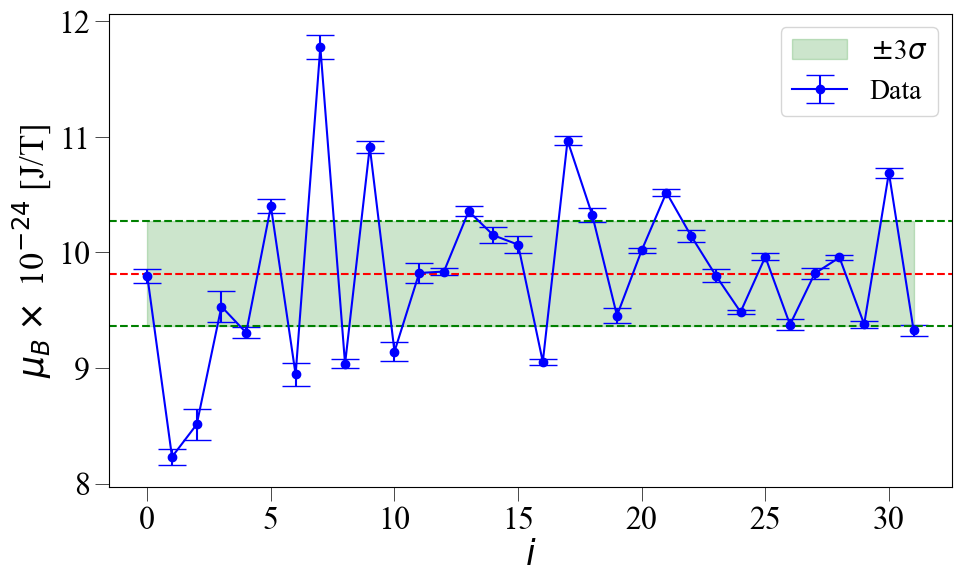
\includegraphics[scale=0.33]{mu}
                \captionsetup{justification=centering, font=footnotesize}
                \captionof{figure}{Hodnoty Bohrova magnetonu $\mu_B$}
                \label{fig:mu}
                \vspace{10pt}
                \raggedright 

            \subsection{Polarizace}
                \par Pro měření polarizace spektrálních čar jsme použili polarizační filtr. Pro normální Zeemanův jev směr šíření světla je kolmý na vektor magnetické indukce. Při natáčení polarizačního filtru o 0° viditelost krajních spektrálních čar je maximální, a viditelost centrální spektrální čáry je minimální. Při natáčení polarizačního filtru o 90° viditelost krajních spektrálních čar je minimální, a viditelost centrální spektrální čáry je maximální. Polarizace je tedy lineární.
                \par Pro případ, kde směr šíření světla byl rovnoběžný se směrem magnetické indukce, použilí jsme čtvrtvlnné destičky, která posouvá fázi o $\delta$=$\pi/2$, před polarizačním filtrem natáčením polarizačního filtru o 45° byl viditelen vnější kroužek. Při natáčení o -45° byl viditelný vnitřní kroužek. To je dáno tím, že po převedení na lineární polarizaci má středová čára opačný směr oproti rozštěpeným čarám, tj. emitované světlo ve směru magnetické indukce je polarizováno lineárně, ale střední spektrální čára má polarizaci kolmo na krajní rozštěpené čáry. Polarizace je tedy kruhová, přičemž jeden typ čar je pravotočivý a druhý levotočivý. Po převedení na lineární polarizaci mají opačný směr.
                \par Při anomálním Zeemanově jevu spektrální čáry jsou rozložené na devět čar kroužků.
    \end{minipage}
\newpage
                \par K výpočtu veličin a jejich nejistot byla použita knihovna Uncertinties pro Python \cite{uncertainties}. Chyby byly rozšířeny o Studentův koeficient (2-Tail Confidence Level) s ohledem na stupně volnosti pro každou hodnotu, pro interval spolehlivosti 99.73\%.

        \section{Závěr}
                Byla ověřena funkce Fabry-Perotova interferometru. Při $B$ = 0 T byla zjištěna hodnota $\alpha$ = 0.081(1) [1/mm$^2$], což potvrzuje lineární charakter závislosti $r^2$ na pořadí $p$. 
                \par Byla zjištěna hodnota Bohrova magnetonu $\mu_B$ = 9.8(5) $\times 10^{-24}$ [J/T]. Tabulková hodnota Bohrova magnetonu je $\mu_B$ = 9.274 $\times 10^{-24}$ [J/T] \cite{magneton}. Rozdíl mezi tabulkovou hodnotou a hodnotou získanou v experimentu je 0.5(5) $\times 10^{-24}$ [J/T]. Rozdíl je docela malý, což znamená, že hodnoty jsou v souladu.
                \par Byla zjištěna polarizace spektrálních čar. Pro normální Zeemanův jev byla zjištěna lineární polarizace kolmo k magnetické indukci. Při použití čtvrtvlnné destičky z posunem $\delta$=$\pi/2$ byla zjištěna kruhová polarizace ve směru magnetické indukce. 

                \renewcommand{\refname}{Odkazy}
                \begin{thebibliography}{9}
                    \bibitem{uncertainties}
                        Uncertainties, Dostupné online: \url{https://pypi.org/project/uncertainties}
                    \bibitem{magneton}
                        Bohrův magneton, Dostupné online: \url{https://www.vedantu.com/physics/bohr-magneton}
                \end{thebibliography} 

    \begin{center}
        \section{Appendix}
            \subsection{Tabulka naměřené hodnoty poloměrů interferenčních kroužků $r$ při $I$ = 0 A}
                \pgfplotstabletypeset[
                col sep=comma, % Defines the separator, comma for CSV
                string type, % Treats columns as strings (not math mode)
                every head row/.style={before row=\toprule,after row=\midrule},
                every last row/.style={after row=\bottomrule},
                columns/p/.style={column name=$p$},
                columns/r/.style={column name=$r$ [mm]},
                columns/r^2/.style={column name=$r^2$ [mm$^2$]}
                ]{data/B_1_out.csv}
            
            \subsection{Data zavislosti magnetické indukce $B$ na proudu $I$}
                \pgfplotstabletypeset[
                col sep=comma, % Defines the separator, comma for CSV
                string type, % Treats columns as strings (not math mode)
                every head row/.style={before row=\toprule,after row=\midrule},
                every last row/.style={after row=\bottomrule},
                columns/I/.style={column name=$I$ [A]},
                columns/B/.style={column name=$B$ [mT]}
                ]{data/I_B_out.csv}

            \subsection{Tabulka naměřených hodnot Bohrova magnetonu $\mu_B$ pro $I$ = 3.15 A}
                \pgfplotstabletypeset[
                col sep=comma, % Defines the separator, comma for CSV
                string type, % Treats columns as strings (not math mode)
                every head row/.style={before row=\toprule,after row=\midrule},
                every last row/.style={after row=\bottomrule},
                columns/p/.style={column name=$p$},
                columns/r_a/.style={column name=$r_a$ [mm]},
                columns/r_b/.style={column name=$r_b$ [mm]},
                columns/r_c/.style={column name=$r_c$ [mm]},
                columns/mu_ab/.style={column name=$\mu_{B,ab}$ $\times 10^{-24}$[J/T]},
                columns/mu_bc/.style={column name=$\mu_{B,bc}$ $\times 10^{-24}$[J/T]}
                ]{data/B_4_out.csv}

            \subsection{Tabulka naměřených hodnot Bohrova magnetonu $\mu_B$ pro $I$ = 4.13 A}
                \pgfplotstabletypeset[
                col sep=comma, % Defines the separator, comma for CSV
                string type, % Treats columns as strings (not math mode)
                every head row/.style={before row=\toprule,after row=\midrule},
                every last row/.style={after row=\bottomrule},
                columns/p/.style={column name=$p$},
                columns/r_a/.style={column name=$r_a$ [mm]},
                columns/r_b/.style={column name=$r_b$ [mm]},
                columns/r_c/.style={column name=$r_c$ [mm]},
                columns/mu_ab/.style={column name=$\mu_{B,ab}$ $\times 10^{-24}$[J/T]},
                columns/mu_bc/.style={column name=$\mu_{B,bc}$ $\times 10^{-24}$[J/T]}
                ]{data/B_5_out.csv}

            \subsection{Tabulka naměřených hodnot Bohrova magnetonu $\mu_B$ pro $I$ = 4.98 A}
                \pgfplotstabletypeset[
                col sep=comma, % Defines the separator, comma for CSV
                string type, % Treats columns as strings (not math mode)
                every head row/.style={before row=\toprule,after row=\midrule},
                every last row/.style={after row=\bottomrule},
                columns/p/.style={column name=$p$},
                columns/r_a/.style={column name=$r_a$ [mm]},
                columns/r_b/.style={column name=$r_b$ [mm]},
                columns/r_c/.style={column name=$r_c$ [mm]},
                columns/mu_ab/.style={column name=$\mu_{B,ab}$ $\times 10^{-24}$[J/T]},
                columns/mu_bc/.style={column name=$\mu_{B,bc}$ $\times 10^{-24}$[J/T]}
                ]{data/B_6_out.csv}

            \subsection{Tabulka naměřených hodnot Bohrova magnetonu $\mu_B$ pro $I$ = 5.99 A}
                \pgfplotstabletypeset[
                col sep=comma, % Defines the separator, comma for CSV
                string type, % Treats columns as strings (not math mode)
                every head row/.style={before row=\toprule,after row=\midrule},
                every last row/.style={after row=\bottomrule},
                columns/p/.style={column name=$p$},
                columns/r_a/.style={column name=$r_a$ [mm]},
                columns/r_b/.style={column name=$r_b$ [mm]},
                columns/r_c/.style={column name=$r_c$ [mm]},
                columns/mu_ab/.style={column name=$\mu_{B,ab}$ $\times 10^{-24}$[J/T]},
                columns/mu_bc/.style={column name=$\mu_{B,bc}$ $\times 10^{-24}$[J/T]}
                ]{data/B_7_out.csv}

            \subsection{Tabulka naměřených hodnot Bohrova magnetonu $\mu_B$ pro $I$ = 7.19 A}
                \pgfplotstabletypeset[
                col sep=comma, % Defines the separator, comma for CSV
                string type, % Treats columns as strings (not math mode)
                every head row/.style={before row=\toprule,after row=\midrule},
                every last row/.style={after row=\bottomrule},
                columns/p/.style={column name=$p$},
                columns/r_a/.style={column name=$r_a$ [mm]},
                columns/r_b/.style={column name=$r_b$ [mm]},
                columns/r_c/.style={column name=$r_c$ [mm]},
                columns/mu_ab/.style={column name=$\mu_{B,ab}$ $\times 10^{-24}$[J/T]},
                columns/mu_bc/.style={column name=$\mu_{B,bc}$ $\times 10^{-24}$[J/T]}
                ]{data/B_8_out.csv}

            \subsection{Tabulka naměřených hodnot Bohrova magnetonu $\mu_B$ pro $I$ = 8.22 A}
                \pgfplotstabletypeset[
                col sep=comma, % Defines the separator, comma for CSV
                string type, % Treats columns as strings (not math mode)
                every head row/.style={before row=\toprule,after row=\midrule},
                every last row/.style={after row=\bottomrule},
                columns/p/.style={column name=$p$},
                columns/r_a/.style={column name=$r_a$ [mm]},
                columns/r_b/.style={column name=$r_b$ [mm]},
                columns/r_c/.style={column name=$r_c$ [mm]},
                columns/mu_ab/.style={column name=$\mu_{B,ab}$ $\times 10^{-24}$[J/T]},
                columns/mu_bc/.style={column name=$\mu_{B,bc}$ $\times 10^{-24}$[J/T]}
                ]{data/B_9_out.csv}

            \subsection{Tabulka naměřených hodnot Bohrova magnetonu $\mu_B$ pro $I$ = 9.22 A}
                \pgfplotstabletypeset[
                col sep=comma, % Defines the separator, comma for CSV
                string type, % Treats columns as strings (not math mode)
                every head row/.style={before row=\toprule,after row=\midrule},
                every last row/.style={after row=\bottomrule},
                columns/p/.style={column name=$p$},
                columns/r_a/.style={column name=$r_a$ [mm]},
                columns/r_b/.style={column name=$r_b$ [mm]},
                columns/r_c/.style={column name=$r_c$ [mm]},
                columns/mu_ab/.style={column name=$\mu_{B,ab}$ $\times 10^{-24}$[J/T]},
                columns/mu_bc/.style={column name=$\mu_{B,bc}$ $\times 10^{-24}$[J/T]}
                ]{data/B_10_out.csv}
            
            \subsection{Tabulka naměřených hodnot Bohrova magnetonu $\mu_B$ pro $I$ = 9.90 A}
                \pgfplotstabletypeset[
                col sep=comma, % Defines the separator, comma for CSV
                string type, % Treats columns as strings (not math mode)
                every head row/.style={before row=\toprule,after row=\midrule},
                every last row/.style={after row=\bottomrule},
                columns/p/.style={column name=$p$},
                columns/r_a/.style={column name=$r_a$ [mm]},
                columns/r_b/.style={column name=$r_b$ [mm]},
                columns/r_c/.style={column name=$r_c$ [mm]},
                columns/mu_ab/.style={column name=$\mu_{B,ab}$ $\times 10^{-24}$[J/T]},
                columns/mu_bc/.style={column name=$\mu_{B,bc}$ $\times 10^{-24}$[J/T]}
                ]{data/B_11_out.csv}
    \end{center}
\end{document}